\documentclass[./main.tex]{subfiles}

\begin{document}

    
\subsubsection{IoT - základy}

\begin{wrapfigure}{r}{0.55\textwidth}
\centering
  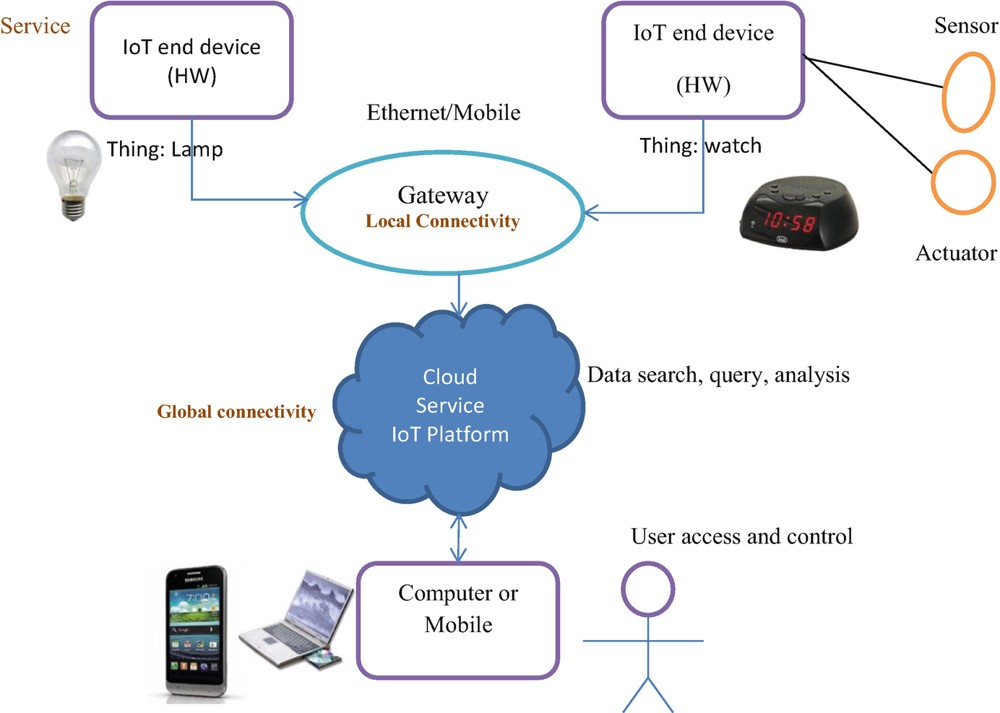
\includegraphics[width=0.5\textwidth]{images/IoT_cloud_platform.png}
  \caption{IoT architektúra s využitím cloudovej
  služby}\cite{springerprofessional.de_The_Era_of_IoT}
  \label{fig:IoT_ARCH_CLOUD}
\end{wrapfigure} 
% Prvýkrát použil slovné spojenie Internet of Things Kevin Ashton, zakladateľ spoločnosti Auto-ID Center v roku 1999. 
% „“ zistit ako sa robia uvodzovky

Výraz \say{Internet of Things} pravdepodobne prvý krát použil  Kevin Ashton
zakladateľ spoločnosti Auto-ID Center v roku 1999 na prezentácii v spoločnosti Procter \& Gamble (P\&G) V USA. Výraz poukazoval na novú RFID technológiu v dopravnom reťazci P\&G. \cite{KODYS, kevinAshton}. Riešenie Internet of Things  -  IoT používa pri implementácií rôzne technológie, ako sú RFID tagy, čiarové kódy, GPS technológie, vozidlá, stroje, predmety so vstavanou elektronikou, senzormi s pripojením na sieť. Úlohou je ovládať pripojené komponenty na diaľku cez existujúce sieťové infraštruktúry a integrácia fyzického sveta\cite{KODYS} do počítačových systémov, pomocou získavania, výmenou, ukladaním a prispôsobením dát. Výsledkom je zvýšenie efektivity, presnosti, ekonomické prínosy \cite{industry4}, Pridaním počítačovej inteligencie k zariadeniu zlepšíme jeho funkciu a pridáme ho k počítačovej sieti. Takýto systém produkuje veľké množstvo dát, ktoré treba analyzovať, spracovať a uložiť. Pre toto spracovanie dát, môžeme rozmýšľať či nevyužijeme cloudovú platformu.\cite{springerprofessional.de_The_Era_of_IoT} %dopln dovod
Na obrázku (Obr.\ref{fig:IoT_ARCH_CLOUD} zo strany \pageref{fig:IoT_ARCH_CLOUD})je zobrazená schéma takejto platformy.
Výraz IoT pokrýva 3 druhy komunikácie, ktoré je možné vytvoriť:\cite{addressing_IoT_ipv6}
%este daco dopisat
\begin{multicols}{3}
    \begin{itemize}
        \item Object-to-Person \item  object-to-object \item machine-to-machine
    \end{itemize}
\end{multicols}






\end{document}